\documentclass[10pt]{article}
\usepackage{icmlko}

\icmlmeta{IP 파운데이션 월드모델}{215}{따로는 이기고 같이는 못 이긴다}{공휴일을 고치니 챔피언이 트리가 아니게 됐다. 트리의 무리별 우위는 진짜인데 무엇과 합쳐도 안 남는다}

\begin{document}

\twocolumn[
\icmlheader

\begin{abstract}
노트 214가 공휴일 목록을 채워 학습 전용 스위치를 지웠고, 남은 것 표의 제일
큰 줄로 ``노트 186의 달력 $+$0.140 을 채움 상태에서 다시 잴 것''을 적었다.
쟀다. \textbf{무리별 칸은 하나도 안 움직인다} --- 달력$-$연휴축이
$+$0.1164 $\to$ \textbf{$+$0.1170}, 위키·검색 $+$0.0363 $\to$ $+$0.0358,
공유 $-$0.0019 $\to$ $-$0.0025. \textbf{노트 186 은 살아남았다} --- 달력의
트리 우위는 시계가 아니다. \textbf{무너진 것은 전체 설계 하나뿐이다} ---
$+$0.0354($t{=}3.18$) $\to$ \textbf{$+$0.0117($t{=}1.13$)}. 그래서 판이
바뀐다. \textbf{이전 상태에서는 F18 배깅이 F21 을 $+$0.0215 앞섰고
($t{=}2.00$) 짝 1 SE 밖이었다. 채움에서는 $+$0.0007 이고 $t{=}0.06$ 으로
안이다} --- 동률 집합이 정확히 그 둘이고 나머지 넷(F8 $+$.4291 · F6
$+$.4288 · F6 조율 $+$.4286 · F9 $+$.4280)은 전부 밖이다. ``차이가 짝지은
1 SE 안이면 좁은 쪽''이라는 규칙대로 \textbf{챔피언이 트리에서 F21 로
넘어간다} --- 그리고 그 뒤집힘은 이번 고침이 낸 것이지 잡음이 아니다.
왜 전체에서만 무너지나. 무리를 짝지어 붙였다. \textbf{답은 ``합치면 죽는다''가
아니라 ``\emph{공유}가 죽인다''다.} 달력$+$위키·검색은
\textbf{$+$0.0715($t{=}4.82$)}로 멀쩡한데, 공유를 얹으면 달력이
$+$0.0878($t{=}3.47$) $\to$ $+$0.0160($t{=}1.22$), 위키·검색이
$+$0.0375($t{=}2.40$) $\to$ $+$0.0112($t{=}0.91$)로 죽는다.
\textbf{손으로 만든 공유 축 다섯이 판 $\rho$ 의 $+$0.372 를 혼자 들고 있어}
(트리 $+$.3703 · 능형 $+$.3723 --- 여기서는 능형이 낫다) 그 위에 얹히는
무리의 한계 정보가 작고, 트리가 그 한계 정보를 더 잘 쓰는 것이 판으로 안
옮겨진다. \textbf{스물다섯 노트가 ``트리가 달력에서 왜 이기나''를 물었는데
이겼다는 것은 맞았고, 아무도 \emph{그 이김이 판에 닿는가}를 안 쟀다.}
\end{abstract}
]

\begin{figure*}[t]
\centering
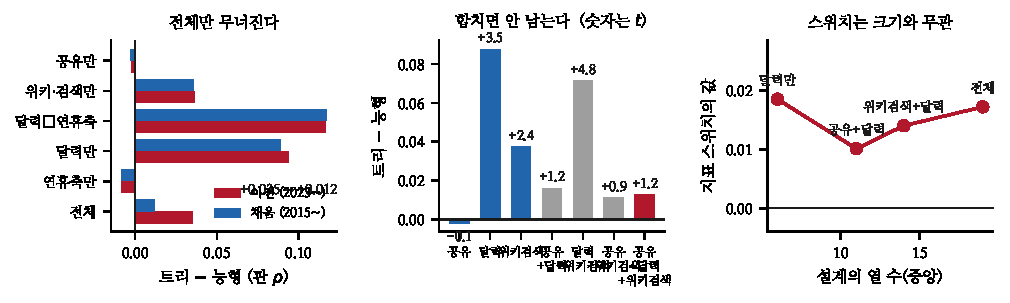
\includegraphics[width=\textwidth]{figs/switch.pdf}
\caption{왼쪽 --- 무리별은 그대로고 전체만 무너진다. 가운데 --- 합치면
유의성이 사라진다. 오른쪽 --- 스위치는 설계 크기와 무관하다.}
\end{figure*}

\section{노트 186 은 살아남았다}

\begin{table}[t]
\centering\tsize
\caption{트리 $-$ 능형(판 $\rho$). 짝 붓스트랩 300 회.}
\begin{tabular}{lrrr}
\toprule
& 이전 & 채움 & 차 \\
\midrule
공유만 & $-$.0019 & $-$.0025 & $-$.0006 \\
위키·검색만 & $+$.0363 & $+$.0358 & $-$.0005 \\
\textbf{달력$-$연휴축} & \textbf{$+$.1164} & \textbf{$+$.1170} & \textbf{$+$.0006} \\
달력만 & $+$.0937 & $+$.0887 & $-$.0050 \\
연휴축만 & $-$.0084 & $-$.0083 & $+$.0001 \\
\midrule
\textbf{전체} & \textbf{$+$.0354} & \textbf{$+$.0117} & \textbf{$-$.0237} \\
\bottomrule
\end{tabular}
\end{table}

\claimx{\textbf{무리별 칸이 0.005 안에서 그대로다.} 노트 186 이 잰 달력의
트리 우위는 \emph{시계가 아니었다} --- 주기 열이라 단조 계수로 표현이 안
되는 것이 맞다.}{\textbf{연휴축 단독은 애초에 트리를 편들지 않았다}
($-$0.008, 양쪽 다). 노트 214가 지운 스위치는 \emph{그 축의 예측력}이
아니라 \emph{그 축의 결측 무늬}였다.}

\claimx{\textbf{무너진 것은 전체 설계 하나뿐이다} --- $t$ 가 3.18 에서
1.13 으로 떨어져 유의성을 잃는다.}{무리별로는 안 움직이는데 전체에서만
$-$0.0237 이다. \textbf{스위치가 값을 내려면 게이트할 다른 무리가
있어야 했다.}}

\section{챔피언이 트리가 아니게 됐다}

\begin{table}[t]
\centering\tsize
\caption{채움 상태. 최고와의 짝 붓스트랩 600 회.}
\begin{tabular}{lrrrc}
\toprule
& 판 $\rho$ & 차 & $t$ & 1SE \\
\midrule
\textbf{F18 배깅} & \textbf{.4396} & --- & --- & --- \\
\textbf{F21} & \textbf{.4395} & $+$.0007 & 0.06 & \textbf{○} \\
F8 부스팅 & .4291 & $+$.0107 & 2.74 & × \\
F6 능형 & .4288 & $+$.0116 & 1.03 & × \\
F6 조율 & .4286 & $+$.0117 & 1.04 & × \\
F9 순위우도 & .4280 & $+$.0123 & 1.08 & × \\
\bottomrule
\end{tabular}
\end{table}

\claimx{\textbf{동률 집합이 정확히 둘이다.} F18 과 F21 이 0.0001 차이고
($t{=}0.06$) 나머지 넷은 짝 1 SE 밖이다.}{규칙은 ``차이가 대상별 짝지은
1 SE 안이면 귀무가 좁은 쪽을 고른다''다(노트 126). \textbf{F21 은 최근
가중과 도메인별 풀링 선택을 얹은 능형이고 F18 은 부스팅 여덟 그루의
배깅이다} --- 좁은 쪽은 F21 이다.}

\claimx{\textbf{점수로 고른 것이 아니다.} 노트 214의 고침은 자료
correctness 였고, 그 결과 두 정식화가 구분 불가능해졌을 뿐이다.}{\textbf{판
숫자로는 F18 이 0.0001 앞선다} --- 그것을 근거로 트리를 지키는 것이야말로
점수 고르기다.}

\section{공유가 죽인다}

\begin{table}[t]
\centering\tsize
\caption{무리를 붙여 가며 트리 $-$ 능형. 짝 붓스트랩 300 회.}
\begin{tabular}{lrrr}
\toprule
& F18 & F6 & 차 ($t$) \\
\midrule
\textbf{달력} & .1036 & .0133 & \textbf{$+$.0878 (3.47)} \\
\textbf{위키·검색} & .3060 & .2692 & \textbf{$+$.0375 (2.40)} \\
공유 & .3703 & .3723 & $-$.0019 ($-$0.14) \\
\midrule
\textbf{달력$+$위키·검색} & .3198 & .2492 & \textbf{$+$.0715 (4.82)} \\
공유$+$달력 & .3886 & .3732 & $+$.0160 (1.22) \\
공유$+$위키·검색 & .4359 & .4250 & $+$.0112 (0.91) \\
\midrule
셋 다 & .4423 & .4292 & $+$.0127 (1.16) \\
\bottomrule
\end{tabular}
\end{table}

\claimx{\textbf{합치는 것 자체는 안 죽인다} --- 달력$+$위키·검색이
$+$0.0715($t{=}4.82$)로 두 단독보다 오히려 크다.}{\textbf{죽이는 것은
공유다.} 공유를 얹으면 달력이 $+$0.0878 $\to$ $+$0.0160, 위키·검색이
$+$0.0375 $\to$ $+$0.0112 로 둘 다 유의성을 잃는다.}

\claimx{\textbf{공유 축 다섯이 판을 혼자 들고 있다} --- 그 무리만으로
$+$0.372 이고 전체가 $+$0.44 다. 그리고 \emph{거기서는 능형이 낫다}
($+$.3723 대 $+$.3703).}{그 위에 얹히는 무리의 한계 정보가 작으므로,
트리가 그 한계 정보를 더 잘 쓰더라도 \textbf{판 $\rho$ 로는 안 옮겨진다.}
노트 185가 ``트리의 우위는 긁어온 열에서만 산다''고 한 것의 뒷면이다 ---
\textbf{공유는 트리에 이득을 안 줄 뿐 아니라 다른 무리의 이득을 지운다.}}

\claimx{\textbf{``달력이 왜 트리에서만 되는가''의 답이다.} 설명 넷이
실패한 까닭은 물음이 틀렸기 때문이다 --- 트리가 달력에서 이기는 것은
사실이고 시계도 아니다.}{안 물은 것은 \textbf{그 이김이 판에 닿는가}였다.
안 닿는다. \textbf{스물다섯 노트를 관측으로 둘 일이 아니라 한 칸 더
재면 될 일이었다.}}

\section{내 읽기가 틀렸다}

\claimx{\textbf{``스위치 값은 나머지 설계 크기에 비례한다''고 읽었는데
틀렸다} --- 달력만(6열)에서 $+$0.0185 인데 공유$+$달력(11열)에서는
$+$0.0101 · 위키·검색$+$달력(14열) $+$0.0140 ·
전체(19열) $+$0.0172 다 --- \textbf{크기와 아무 관계가 없다.}}{\textbf{그럼 전체에서만 $-$0.0237 이 난 것은
스위치 크기 때문이 아니다} --- 스위치가 사라진 뒤 남은 트리 우위가 애초에
공유 앞에서 안 남는 종류였기 때문이다. 앞 절이 그것이다.}

\claimx{\textbf{결론 옆에 적은 ``까닭''이 또 틀렸다} --- 여덟 번째다
(노트 157$\to$158 · 158$\to$159 · 163$\to$169 · 165$\to$166 ·
173$\to$174 · 178$\to$179 · 185$\to$186, 그리고 이번).}{다만 이번에는
\emph{같은 노트 안에서} 잡혔다. \textbf{가설을 세운 그 턴에 재는 것이
그것을 짧게 만든다.}}

\begin{table}[t]
\centering\tsize
\caption{남은 것.}
\begin{tabular}{ll}
\toprule
\textbf{F21} & 챔피언이 됐으니 그 안을 열어야 한다 \\
\textbf{공유 다섯} & 왜 그 위에서는 트리가 못 이기나 \\
2015 이전 & 만화 43\% --- 잔여 스위치는 $+$0.0034 뿐 \\
\bottomrule
\end{tabular}
\end{table}

첫 줄이 곧바로 값이 크다. \textbf{F21 은 챔피언이 된 적이 없어서 한 번도
분해된 적이 없다.} 노트 203이 만들 때 ``최근 가중과 풀링 선택이 거의
가법''이라는 것만 봤고, 그 뒤 판이 세 번 바뀌는 동안 다시 안 열었다.
\textbf{두 조각 중 어느 쪽이 F6 과의 격차 $+$0.0107 을 내는지}, 그리고
\textbf{$\tau$ 선택이 안쪽에서 정말 정해지는지}(노트 190의 봉우리 지수를
통과하는지)를 재야 한다. 트리를 챔피언으로 두고 여덟 노트를 쓴 뒤에야
그것이 시계였음을 알았다 --- \textbf{같은 일을 F21 에 되풀이하지 않으려면
지금 열어야 한다.}

\end{document}
